% fig_mkip: multidimensional knapsack interdiction on a toy instance with two resources.
% 6 items (profit p, weight w, volume v); the follower's knapsack takes at most weight 8
% and volume 10; the leader may block 2 items (each block costs 1, budget 2).
% Data (checked by brute force over all 15 pairs of blocked items and every packing):
%   p = 6 9 4 5 8 6,  w = 2 3 3 2 3 3,  v = 2 3 3 3 5 4,  W = 8, V = 10.
%   No blocking: the follower packs items 1,2,5 (1-based): value 23, weight 8, volume 10.
%   Best blocking: items 1 and 2 (p 6 and 9); the follower's best packing of the rest is
%   items 3,4,6: value 4+5+6 = 15, weight 3+2+3 = 8, volume 3+3+4 = 10 (both limits
%   reached; unique).  Next best pairs leave 17 ({1,4} and {2,5}); blocking the two most
%   valuable items (9 and 8, items 2 and 5) leaves 17.  With the weight limit alone the
%   best pairs would be {1,4} and {2,5} (value 17), so the volume limit changes the answer.
% Build: pdflatex fig_mkip.tex   (6.5 in x 1.9 in)
\documentclass[tikz,border=2pt]{standalone}
\pdfinfoomitdate=1 \pdftrailerid{} \pdfsuppressptexinfo=-1 % byte-identical rebuilds
\usepackage{mathptmx}
\usetikzlibrary{arrows.meta,calc}
\definecolor{leader}{HTML}{2A78D6}
\definecolor{follower}{HTML}{EB6834}
\definecolor{cert}{HTML}{1BAF7A}
\definecolor{ink}{HTML}{0B0B0B}
\definecolor{ink2}{HTML}{52514E}
\definecolor{muted}{HTML}{A9A8A2}
\definecolor{grid}{HTML}{E6E5E0}
\tikzset{
  every picture/.style={font=\fontsize{8}{9.6}\selectfont, color=ink, line cap=round},
  wbar/.style={fill=ink2},                                   % weight: solid bar
  vbar/.style={draw=ink2, line width=0.6pt, fill=white},     % volume: open bar
}
\def\u{0.22}   % cm per unit, bars on the cards
\def\cw{1.45}  % card width
\def\ch{1.20}  % card height
\def\cy{2.70}  % bottom of the cards
% \card{left}{profit}{weight}{volume}{state: 0 left, 1 blocked, 2 packed}
\newcommand{\card}[5]{%
  \ifcase#5
    \draw[ink2, line width=0.6pt, fill=white] (#1,\cy) rectangle ++(\cw,\ch);
  \or
    \draw[muted, line width=0.6pt, fill=grid] (#1,\cy) rectangle ++(\cw,\ch);
  \or
    \draw[follower, line width=0.8pt, fill=follower!22] (#1,\cy) rectangle ++(\cw,\ch);
  \fi
  \fill[wbar] (#1+0.17,\cy+0.42) rectangle ++(#3*\u,0.15);
  \draw[vbar] (#1+0.17,\cy+0.16) rectangle ++(#4*\u,0.15);
  \ifnum#5=1
    \draw[ink2, line width=0.9pt] (#1+0.08,\cy+0.08) -- (#1+\cw-0.08,\cy+\ch-0.08)
                                  (#1+0.08,\cy+\ch-0.08) -- (#1+\cw-0.08,\cy+0.08);
    \node[text=ink2, fill=grid, inner sep=1.2pt] at (#1+\cw/2,\cy+0.88) {#2};
  \else
    \node at (#1+\cw/2,\cy+0.88) {#2};
  \fi}
\begin{document}
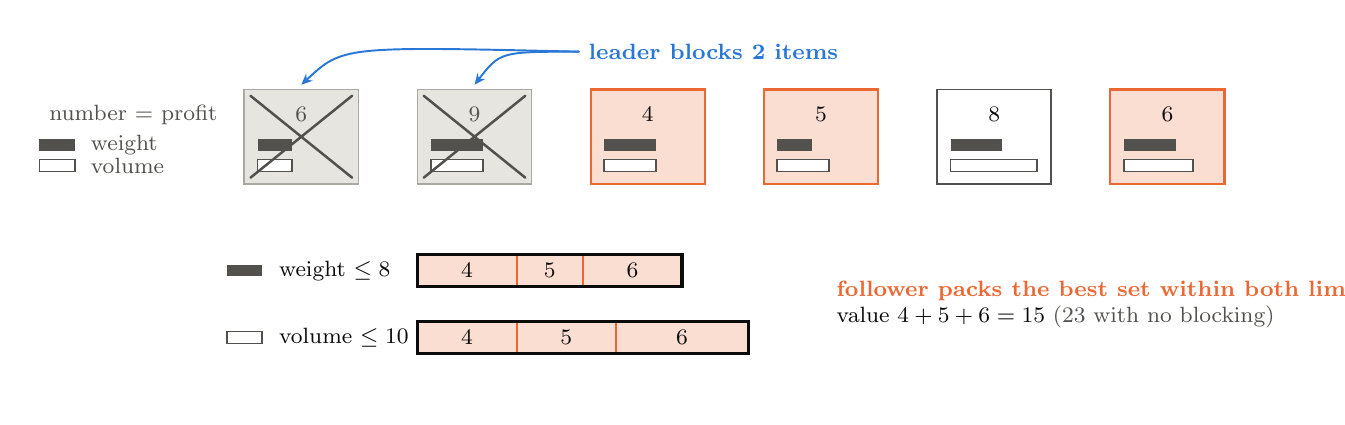
\begin{tikzpicture}
  % fixed page: 6.5 in x 1.9 in including the 2 pt border
  \useasboundingbox (0,0) rectangle (16.37,4.685);

  % ---- the six items: profit, weight bar, volume bar ----
  \card{2.75}{6}{2}{2}{1}
  \card{4.95}{9}{3}{3}{1}
  \card{7.15}{4}{3}{3}{2}
  \card{9.35}{5}{2}{3}{2}
  \card{11.55}{8}{3}{5}{0}
  \card{13.75}{6}{3}{4}{2}

  % ---- key ----
  \node[anchor=west, text=ink2] at (0.15,\cy+0.88) {number = profit};
  \fill[wbar] (0.15,\cy+0.42) rectangle ++(0.45,0.15);
  \node[anchor=west, text=ink2] at (0.68,\cy+0.495) {weight};
  \draw[vbar] (0.15,\cy+0.16) rectangle ++(0.45,0.15);
  \node[anchor=west, text=ink2] at (0.68,\cy+0.235) {volume};

  % ---- leader: blocks 2 items ----
  \node[text=leader, font=\fontsize{8}{9.6}\selectfont\bfseries, anchor=west] (lead) at (7.0,4.38)
    {leader blocks 2 items};
  \draw[leader, line width=0.7pt, -{Stealth[length=4pt,width=3.5pt]}]
    (lead.west) .. controls (6.0,4.38) .. (5.675,\cy+\ch+0.06);
  \draw[leader, line width=0.7pt, -{Stealth[length=4pt,width=3.5pt]}]
    (lead.west) .. controls (4.0,4.45) .. (3.475,\cy+\ch+0.06);

  % ---- follower: one knapsack, two limits ----
  \def\g{0.42}   % cm per unit in the gauges
  \def\gx{4.95}  % left end of the gauges
  \def\gh{0.40}  % gauge height
  % weight: items with profits 4, 5, 6 use 3 + 2 + 3 = 8 of 8
  \def\gy{1.40}
  \foreach \a/\b/\p in {0/3/4, 3/5/5, 5/8/6}
    \draw[follower, line width=0.8pt, fill=follower!22] (\gx+\a*\g,\gy) rectangle (\gx+\b*\g,\gy+\gh)
      node[midway, text=ink] {\p};
  \draw[ink, line width=1.1pt] (\gx,\gy) rectangle (\gx+8*\g,\gy+\gh);
  \fill[wbar] (\gx-2.42,\gy+0.125) rectangle ++(0.45,0.15);
  \node[anchor=west] at (\gx-1.88,\gy+\gh/2) {weight $\le 8$};
  % volume: 3 + 3 + 4 = 10 of 10
  \def\gy{0.55}
  \foreach \a/\b/\p in {0/3/4, 3/6/5, 6/10/6}
    \draw[follower, line width=0.8pt, fill=follower!22] (\gx+\a*\g,\gy) rectangle (\gx+\b*\g,\gy+\gh)
      node[midway, text=ink] {\p};
  \draw[ink, line width=1.1pt] (\gx,\gy) rectangle (\gx+10*\g,\gy+\gh);
  \draw[vbar] (\gx-2.42,\gy+0.125) rectangle ++(0.45,0.15);
  \node[anchor=west] at (\gx-1.88,\gy+\gh/2) {volume $\le 10$};

  \node[anchor=west, align=left] at (10.15,1.17)
    {{\bfseries\color{follower}follower packs the best set within both limits}\\
     value $4+5+6 = 15$ \textcolor{ink2}{(23 with no blocking)}};
\end{tikzpicture}
\end{document}
